\chapter{SWOT}
SWOT analysis is one of the most commonly used marketing strategies. 
The analysis identifies strengths, opportunities, and weaknesses and threats~\ref{swot-ref}.
It's also important to use the information gathered in the SWOT analysis to form project objectives and long term goals. 
The following SWOT analysis will be brief and will not go into detail. 
\vspace{\secspace}

\begin{figure}[H]
    \centering
    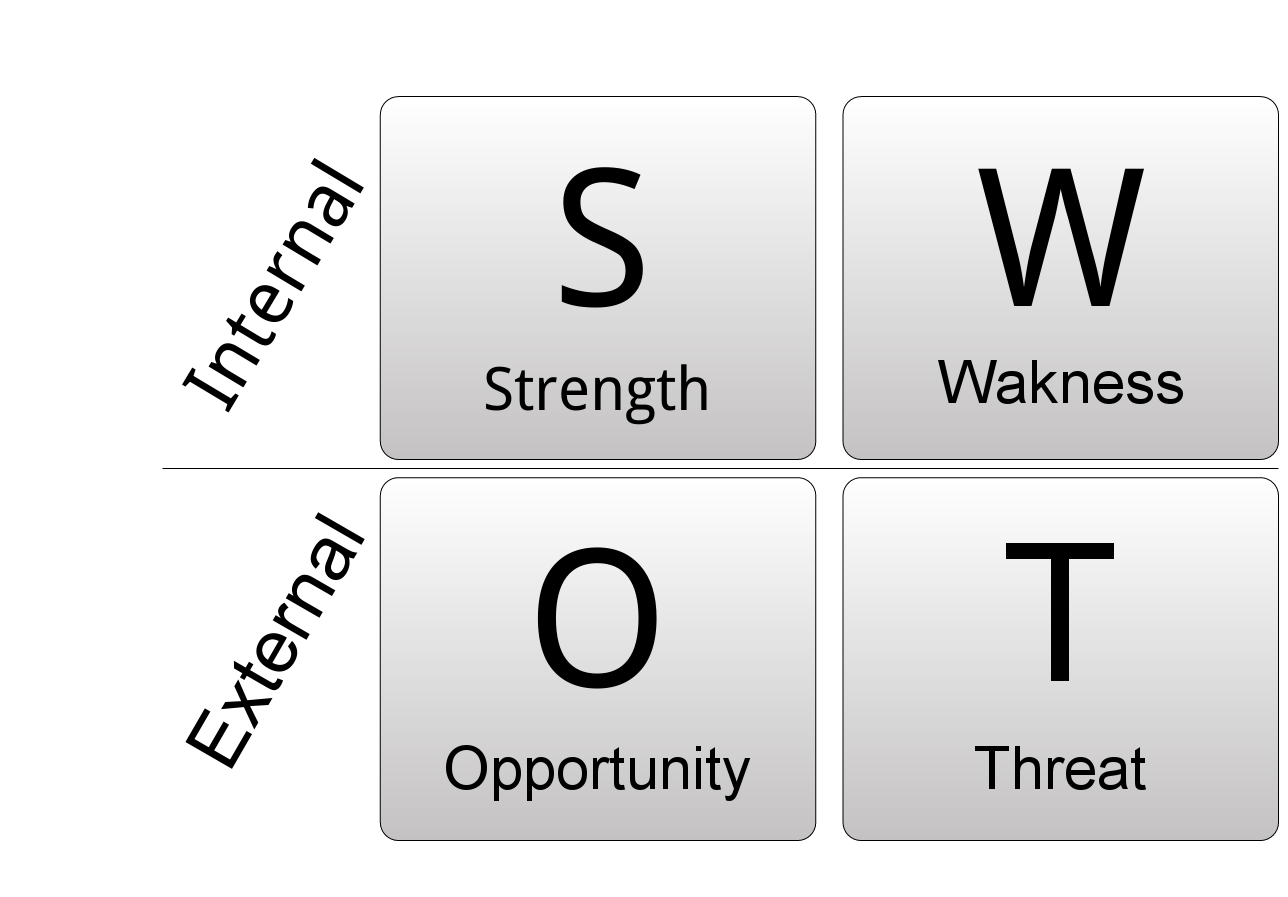
\includegraphics[width=0.6\textwidth]{graphics/swot.png}	
    \caption{SWOT}
    \label{fig:sw}
\end{figure}

\textbf{\Large Strengths}
\begin{itemize}
	 \item Everything is built on already existing technologies
	 \item Module based, which means easy to expand
	 \item Relatively cheap hardware and free software
\end{itemize}

\textbf{\Large Weaknesses}
\begin{itemize}
	 \item Latency caused by HTTP limitations
	 \item Limited to the dynamixel servos (possible to support more manufacturers)
	 \item No team to take the project further
\end{itemize}

\textbf{\Large Opportunities}
\begin{itemize}
	 \item No universal platform (that we could find) exists
	 \item Many different solutions have been tried, but no module based and easy to develop
\end{itemize}

\textbf{\Large Threats}
\begin{itemize}
	 \item Existing technologies doesn't allow easy expansion, but there are many good solutions for different specific tasks
	 \item Marketing problems 
     \item End of EiT
\end{itemize}

As described above the project has a relatively high degree of innovation. 
This means that there are no similar systems which are based on the same simple principles as this project. 
This may be a result of manufacturers often tends to over-complicate things. 
Its weaknesses are not significant as they can be fixed with a small amount of invested time. 
The one thing really standing in the way of this project is the end of EiT, and the fact that the group is being dissolved. 
